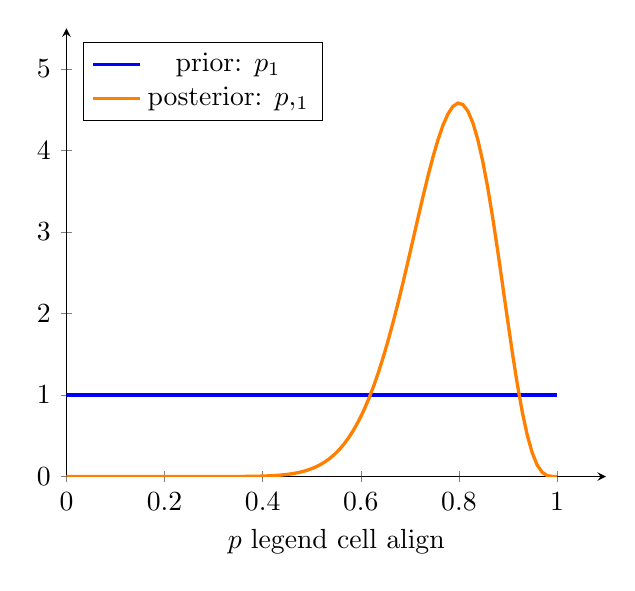
\begin{tikzpicture}[
    declare function={%
      beta(\p,\d,\n)=\p^\d * (1-\p)^(\n-\d) /factorial(\d)/factorial(\n-\d)*factorial(\n+1);
    }
  ]

  \begin{axis}[
      axis lines=left,           % Don't draw box axes
      enlargelimits=upper,       % Extend arrows a little way
      ymax=5,                    % to ensure number 5 is included
      samples=100,               % any fewer and it looks weird
      domain=0:1,                % x range
      xlabel=$p$                 % x label
      legend cell align=left,    % align legend text left
      legend pos= north west,    % put legend in top left
    ]

    \def\pdata{16}    % Number of heads
    \def\pnumber{20}  % Number of coin flips

    % Draw the prior
    \addplot [very thick,blue] {1}; 
    % Add the prior legend
    \addlegendentry{prior: $\Probc{p}{\model_1}$}

    % Draw the posterior
    \addplot [very thick,orange] {beta(x,\pdata,\pnumber)}; 
    % Add the posterior legend
    \addlegendentry{posterior: $\Probc{p}{\data,\model_1}$}

  \end{axis}
\end{tikzpicture}
